%% =====================================================================
%% Overload as a Cusp Catastrophe
%% IEEE conference format (IEEEtran).  Compile:
%%     pdflatex main && bibtex main && pdflatex main && pdflatex main
%% =====================================================================
\documentclass[conference]{IEEEtran}

\usepackage{amsmath,amssymb,amsthm}
\usepackage{graphicx}
\usepackage{booktabs}
\usepackage{url}
\usepackage[hidelinks]{hyperref}
\usepackage{siunitx}

\graphicspath{{../figures/}}

\newtheorem{proposition}{Proposition}
\newtheorem{definition}{Definition}

\DeclareMathOperator{\Var}{Var}
\DeclareMathOperator*{\argmin}{arg\,min}
\newcommand{\dd}{\mathrm{d}}
\newcommand{\Bidx}{\mathcal{B}}

\begin{document}

\title{Overload as a Cusp Catastrophe: Derived Scaling Laws for
Sensory--Executive Tipping Points, and a Ground-Truth Failure of Standard
Early-Warning Indicators}

\author{\IEEEauthorblockN{Neil Thomas Mathew}
\IEEEauthorblockA{Department of Computer Applications\\
CHRIST (Deemed to be University)\\
Bengaluru, India\\
ORCID: 0009-0001-8802-7376}}

\maketitle

% =====================================================================
\begin{abstract}
Sensory and executive overload is usually modelled descriptively: states are
labelled, transitions counted, delayed recovery reported as an asymmetry. Such
models cannot be falsified. We derive overload instead from the geometry of a
cusp catastrophe. A latent load coordinate relaxes in a quartic potential whose
asymmetry is set by demand and whose bistability is set by a slow recovery-debt
variable; functional states become the metastable basins of that potential, and
the transition kernel follows from Kramers escape rates. The formulation fixes
two exponents in advance: hysteresis width
scales as the $3/2$ power of the splitting factor, and near the fold variance
and log-autocorrelation scale as $\mp1/2$ in distance to the tipping point.
Estimation is exact: conditional on the slow variable the drift is linear in a
reparameterised coefficient vector. We report three findings, two about
method. First, on near-unit-root series like tonic electrodermal activity the
nominal test for the cubic term rejects $42\%$ of random walks rather than
$5\%$. Second, the rolling-window indicators the early-warning literature
relies on return exponents of the \emph{wrong sign} on data simulated from a
model that genuinely contains a fold, in all twelve configurations tested,
because the relaxation time outgrows the window exactly where the effect is
largest; we withdraw our own early-warning test as uninterpretable. Third,
across 147 recordings from 40 people, no cusp signature exceeds the calibrated
null, which power bounds to excluding strong and moderate dynamics only. The
work is motivated by autistic adults; none are analysed here.
\end{abstract}

\begin{IEEEkeywords}
Critical transitions, cusp catastrophe, hysteresis, early-warning signals,
electrodermal activity, wearable sensing, state-transition models, sensory
overload, executive function.
\end{IEEEkeywords}

% =====================================================================
\section{Introduction}

Autistic adults frequently describe functional breakdown under combined sensory
and cognitive demand as something that arrives suddenly and departs slowly
\cite{maclennan2022}. Qualitative accounts are consistent on two points that
any adequate model must reproduce: the onset is abrupt rather than
proportional, and recovery outlasts the removal of the load that caused it.
Empirical work supports the coupling that would produce this, with sensory
atypicalities and executive difficulty repeatedly found to co-vary in adult
samples \cite{kiep2025,demetriou2018,demetriou2019}.

Formal models have not kept pace. Computational accounts of autism have been
dominated by Bayesian and predictive-coding framings \cite{pellicano2012},
whose empirical support a ten-year review found mixed and methodologically
inconsistent \cite{chrysaitis2023}, and which are in any case formulated at the
group level over static perceptual inference rather than over the minute-scale
functional dynamics at issue. The most recent dynamical treatment of autism
symptom trajectories is explicitly theoretical, deriving parameter ranges from
the literature and collecting no empirical data \cite{adamou2026}. Meanwhile
the applied literature on state-transition modelling typically assigns discrete
states from experimental condition labels and estimates a transition matrix by
counting. That procedure is close to circular: the recovered matrix largely
re-describes the block structure of the protocol, and it makes no prediction
that could turn out to be wrong.

\subsection*{The shift this paper makes}

We do not posit states and fit transitions between them. We posit a
one-dimensional stochastic relaxation in a cusp potential and let everything
else follow. The load coordinate $x_t$ sits in
$V(x;a,b)=\tfrac14 x^4-\tfrac12 a x^2-bx$, where the \emph{normal factor} $b_t$
carries instantaneous demand and the \emph{splitting factor} $a_t$ carries
depleted regulatory capacity. The substantive claim is that regulatory capacity
does not add to load---it changes the geometry. Below a critical $a$, load
tracks demand smoothly and returns; above it a second attractor appears and the
system acquires a fold, a hysteresis loop, and critical slowing down. Abrupt
onset and slow recovery stop being observations to be reported and become
consequences to be checked.

Because the geometry is closed-form, the consequences are quantitative. The
hysteresis width is not merely positive but proportional to $a^{3/2}$; the
variance of the load near the fold does not merely rise but rises as
$\mu^{-1/2}$ in the distance $\mu$ to the tipping point. These are point
hypotheses about exponents, and they can fail.

\subsection*{Contributions}

\begin{enumerate}
\item A cusp-catastrophe formulation of sensory--executive overload
  (Sec.~\ref{sec:model}) in which the discrete functional states are the
  metastable basins of a fitted potential, and the $5\times5$ transition kernel
  is generated by Kramers escape rates from nine interpretable parameters
  rather than by twenty counted frequencies. The states \emph{stuck} and
  \emph{recovering}, which qualitative work describes but no model defines,
  acquire exact geometric definitions.
\item Two closed-form scaling laws --- hysteresis width $\propto a^{3/2}$
  (Prop.~\ref{prop:hyst}) and early-warning exponents $-1/2$ and $+1/2$
  (Prop.~\ref{prop:ews}) --- stated before estimation and tested as point
  hypotheses with bootstrap confidence intervals.
\item An exact estimator. Conditional on the slow variable the drift is linear
  in a reparameterised coefficient vector, so fitting reduces to profiled
  ordinary least squares over a single scalar: no bounds, no starting values,
  no local optima (Sec.~\ref{sec:estimation}).
\item A quantified warning about inference in this setting. On near-unit-root
  physiological series the nominal test for the governing cubic coefficient
  rejects $42\%$ of random walks rather than $5\%$. Persistent
  series look bimodal and prefer flat-bottomed potentials simply by wandering,
  so matched unit-root surrogates, not nominal distributions and not the nested
  monostable restriction, must be the reference (Sec.~\ref{sec:nulls}).
\item A ground-truth validation of the early-warning toolkit itself, which it
  fails. Rolling-window autocorrelation and variance do not recover the
  predicted exponents on series simulated from a model that genuinely contains
  a fold; they return the wrong sign, at every window length and detrending
  choice tested, because the relaxation time diverges past the window exactly
  where the effect is strongest (Sec.~\ref{sec:ews-invalid}). We accordingly
  withdraw our own early-warning test rather than report an uninterpretable
  number.
\item A bounded null. Across 147 recordings from 40 people in three open
  corpora forming a gradient from fully controlled to fully naturalistic, the
  cusp signature is not detected above the calibrated null --- including a case
  where the marginal distribution is decisively bimodal while the dynamics are
  not bistable, which is precisely the configuration that misleads a study
  reporting only distributional evidence (Sec.~\ref{sec:results}). Of the five
  pre-stated predictions only one proves evaluable with these data and
  instruments; we say which, and why, rather than reporting four numbers that
  would look like tests.
\end{enumerate}

We report the null as the result rather than searching for a subgroup or a
transformation in which the predictions survive. The predictions were stated
before estimation, and the estimator's power to detect the effect was
established before the data were fitted; retrofitting either would forfeit
exactly the property that makes the formulation worth having.

\subsection*{A statement about scope}

The research programme this work belongs to targets autistic adults. None of
the three corpora analysed here contains autistic participants, and no claim
about autistic adults is made from them. Systematic reviews confirm that no
public wearable dataset of autistic adults exists at the temporal density this
model requires \cite{cano2024,chen2025ema}; the closest candidate
\cite{scheeren2025} has released pre-registration materials but not raw data,
and no autism-specific dense series appears in the open experience-sampling
index \cite{siepe2026}.
Section~\ref{sec:protocol} specifies the pre-registered protocol under which
the predictions would transfer, and states in advance what would falsify them.
We consider it better to publish a mechanism with an honest scope than to title
a paper after a population it does not measure.

% =====================================================================
\section{Related Work}

\subsection{Sensory--executive coupling in autistic adults}
Meta-analytic evidence establishes executive difficulty as a replicable feature
of autism \cite{demetriou2018,demetriou2019}, and adult cohorts couple it to
sensory atypicality with large effect sizes \cite{kiep2025,auge2025}.
Qualitative work is the most directly relevant to the present model:
MacLennan \emph{et al.} \cite{maclennan2022} describe overload not as an
instantaneous event but as a staged cascade ending in shutdown, with recovery
extending well past the removal of the trigger. That description is a
qualitative statement of hysteresis, and it is what motivates modelling
capacity as a bifurcation parameter rather than as an additive term.

\subsection{Computational models of autism}
Bayesian and predictive-coding accounts \cite{pellicano2012,arthur2023}
explain perceptual atypicality elegantly but are static and group-level; the
supporting evidence is inconsistent across paradigms \cite{chrysaitis2023}.
Adamou \emph{et al.} \cite{adamou2026} give continuous differential equations
for symptom-domain trajectories across the lifespan, deriving parameters from
theory and collecting no data. The present work differs on all three axes:
discrete metastable states rather than continuous symptom scores, minute-scale
functional dynamics rather than lifespan trajectories, and parameters estimated
from physiological time series rather than assumed.

\subsection{Catastrophe theory in behavioural science, and its bad reputation}
The cusp is the canonical two-control-parameter singularity \cite{thom1975,
gilmore1981} and has an established behavioural-science lineage
\cite{zeeman1976}, most rigorously in van der Maas and Molenaar's treatment of
stagewise cognitive development \cite{vandermaas1992} and in the estimation
machinery of Grasman \emph{et al.} \cite{grasman2009}. That literature fits the
cusp to \emph{cross-sectional} response distributions. The complementary
tradition of recovering latent discrete states from behavioural time series by
hidden Markov modelling \cite{li2023,eisenberg2019} is closer to our
data setting but assumes the states rather than deriving them from a
potential. We use it dynamically:
the potential governs a time series, and the catastrophe flags are tested as
temporal scaling laws rather than as distributional shape statistics.

We should be direct about why that distinction matters. Applied catastrophe
theory acquired a poor reputation for good reason: Zahler and Sussmann
\cite{zahler1977,sussmann1978} showed that many 1970s applications identified
qualitative resemblances between data and cusp cartoons, chose control
parameters post hoc, and stated no prediction that observation could
contradict. Any sufficiently flexible geometry can be made to resemble
anything. That critique applies in full force to a paper that merely asserts
overload ``is'' a cusp.

Our defence is not that the critique has aged out; it is that this paper is
constructed to be vulnerable to it. The control parameters are fixed in advance
by measurement rather than chosen to fit. The predictions are exponents,
$3/2$ and $\mp1/2$, stated before estimation. And the null against which they
are tested is calibrated by simulation rather than assumed. A qualitative
resemblance argument cannot fail; an exponent with a bootstrap confidence
interval can, and in Sec.~\ref{sec:results} it does.

\subsection{Critical transitions and early-warning signals}
Approaching a fold, the leading eigenvalue of the linearised dynamics goes to
zero, so perturbations decay ever more slowly \cite{wissel1984}; the resulting
rise in autocorrelation and variance is the standard early-warning indicator
\cite{scheffer2009,scheffer2012,dakos2012}, and has been applied to depression
\cite{leemput2014,wichers2020,smit2025} and reviewed critically for
psychopathology \cite{helmich2021}. The sceptical literature is equally
important here: Ditlevsen and Johnsen \cite{ditlevsen2010} and Boettiger and
Hastings \cite{boettiger2012} show that rolling-window indicators generate
spurious trends on autocorrelated data and that detection power is often far
lower than reported. Our response is to predict the \emph{exponent} rather than
the direction, and to benchmark against unit-root surrogates.

\subsection{Wearable sensing of autonomic load}
Electrodermal activity indexes sympathetic arousal with a slow tonic and a fast
phasic component \cite{boucsein2012,benedek2010,greco2016cvxeda,
posadaquintero2020}; cardiac variability indexes regulatory capacity
\cite{shaffer2017}. Open corpora \cite{schmidt2018wesad,amin2022exam,
hosseini2022nurse} make idiographic modelling feasible. We exploit the
separation between these sensors to keep the load coordinate and its drivers
measurement-independent (Sec.~\ref{sec:sensors}).

% =====================================================================
\section{The Cusp-Hysteretic Markov Model}
\label{sec:model}

\begin{figure*}[t]
\centering
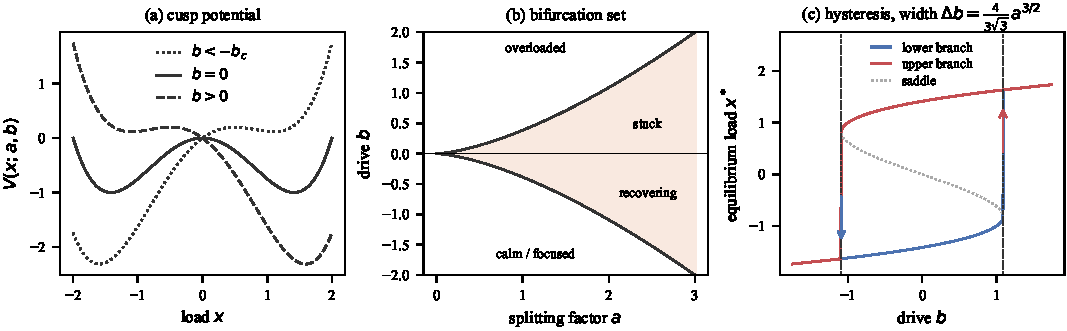
\includegraphics[width=\textwidth]{fig1_geometry}
\caption{The geometry everything else follows from. (a) The cusp potential at
three levels of drive $b$; (b) the bifurcation set in the $(a,b)$ plane, with
the five functional states as regions rather than labels; (c) the hysteresis
loop, whose width is fixed by \eqref{eq:hyst} rather than merely being
positive.}
\label{fig:geometry}
\end{figure*}

\subsection{Latent load in a cusp potential}

Let $x_t\in\mathbb{R}$ be a latent functional-load coordinate, increasing
towards overload. We posit gradient relaxation with additive noise,
\begin{equation}
\dd x_t \;=\; \lambda\Big[-x_t^{3}+a_t x_t + b_t\Big]\dd t \;+\;\sigma\,\dd W_t,
\label{eq:sde}
\end{equation}
the gradient flow of the cusp potential
$V(x;a,b)=\tfrac14x^4-\tfrac12ax^2-bx$. The rate $\lambda>0$ sets the timescale
only; every geometric quantity below depends on $(a,b)$ alone. The control
parameters are linked to observables by
\begin{align}
b_t &= \beta_0+\beta_S S_t+\beta_T T_t+\beta_U U_t, \label{eq:drive}\\
a_t &= \alpha_0+\alpha_A A_t, \label{eq:split}
\end{align}
with $S_t$ sensory-arousal drive, $T_t$ task/behaviour switching cost, $U_t$
contextual uncertainty, and $A_t$ the slow variable defined next.

\subsection{Recovery debt as a slow variable}

\begin{equation}
\dd A_t=\varepsilon\big[\,\mathrm{sp}(x_t-x_{\mathrm{ref}})-A_t\,\big]\dd t,
\qquad \varepsilon\ll1,
\label{eq:slow}
\end{equation}
where $\mathrm{sp}$ is a softplus. Load above baseline accrues debt; debt
decays on timescale $1/\varepsilon$. Through \eqref{eq:split} this debt widens
the hysteresis loop, so an overload episode makes the next one easier --- a
mechanistic reading of the refractory period reported clinically
\cite{maclennan2022}. Note the structural consequence: $(x_t,A_t)$ is Markov,
but the observable state sequence alone is not, because $A_t$ carries history.
This is a testable claim, not a modelling convenience
(Prop.~\ref{prop:dwell}).

\subsection{Folds, thresholds, and the $3/2$ law}

Equilibria solve $x^3-ax-b=0$, whose discriminant we call the
\emph{bistability index}
\begin{equation}
\Bidx_t \;=\; 4a_t^{3}-27b_t^{2},
\label{eq:bistab}
\end{equation}
positive exactly when two stable basins coexist. Folds occur where
$V''(x)=3x^2-a=0$, i.e. at $x_\pm=\pm\sqrt{a/3}$, giving critical drives
$\pm b_c(a)$ with $b_c(a)=\tfrac{2}{3\sqrt3}a^{3/2}$ for $a>0$.

\begin{proposition}[Hysteresis scaling]
\label{prop:hyst}
For $a>0$ the system jumps to the upper branch at $b=+b_c(a)$ and returns at
$b=-b_c(a)$, so the hysteresis loop has width
\begin{equation}
\Delta b(a)\;=\;\frac{4}{3\sqrt3}\,a^{3/2},
\label{eq:hyst}
\end{equation}
and $\Delta b=0$ for $a\le0$.
\end{proposition}

\noindent This is prediction \textbf{P1}. It says more than ``recovery is
delayed'': it fixes the exponent at $3/2$, so a log--log regression of measured
loop width on estimated splitting factor has a predicted slope that the data
can contradict.

\subsection{Early-warning signals, derived}

Linearising \eqref{eq:sde} about a stable equilibrium $x^\ast$ gives relaxation
rate $\lambda_{\mathrm{rel}}=V''(x^\ast)=3x^{\ast2}-a$ and an
Ornstein--Uhlenbeck approximation with
\begin{equation}
\mathrm{AC1}(\Delta t)=e^{-\lambda_{\mathrm{rel}}\Delta t},
\qquad
\Var(x)=\frac{\sigma^{2}}{2\lambda_{\mathrm{rel}}}.
\label{eq:ou}
\end{equation}
At a fold $x^\ast\to\sqrt{a/3}$ and $\lambda_{\mathrm{rel}}\to0$: critical
slowing down is a theorem here, not a postulate.

\begin{proposition}[Early-warning exponents]
\label{prop:ews}
Let $\mu=b_c(a)-b$ be the distance to the upward fold. Near the fold the normal
form gives $\lambda_{\mathrm{rel}}\propto\mu^{1/2}$, hence
\begin{equation}
\Var(x)\propto\mu^{-1/2},
\qquad
-\log\mathrm{AC1}\propto\mu^{+1/2}.
\label{eq:exponents}
\end{equation}
\end{proposition}

\noindent This is prediction \textbf{P2}. The contrast with standard practice
matters: reporting that variance is higher before a transition than in a
control window is weak evidence, because almost any nonstationarity produces
it \cite{ditlevsen2010,boettiger2012}. Predicting $-1/2$ is a point hypothesis.

\subsection{From the diffusion to a hysteretic transition kernel}

In the bistable regime, basin changes are noise-induced escapes over the saddle
$x_s$, with Kramers rate \cite{kramers1940,gardiner2009}
\begin{equation}
r_{i\to j}
=\frac{\sqrt{|V''(x_i^\ast)V''(x_s)|}}{2\pi}
\exp\!\left(-\frac{2\,\Delta V_{i\to j}}{\sigma^{2}}\right),
\label{eq:kramers}
\end{equation}
$\Delta V_{i\to j}=V(x_s)-V(x_i^\ast)$, and discrete-time probability
$P_{ij}=1-\exp(-r_{i\to j}\Delta t)$.

\begin{proposition}[Generated kernel]
\label{prop:kernel}
The $5\times5$ transition matrix is a deterministic function of $(a_t,b_t,
\sigma)$ through \eqref{eq:kramers}, hence of the nine parameters
$(\beta_0,\beta_S,\beta_T,\beta_U,\alpha_0,\alpha_A,\lambda,\sigma,
\varepsilon)$ evaluated at the current covariates. It is non-homogeneous in
time and history-dependent through $A_t$.
\end{proposition}

\noindent A counted homogeneous chain over five states has twenty free
probabilities and cannot depend on covariates at all. Here twenty numbers are
generated by nine, and they move with demand.

\subsection{The five states, derived rather than assigned}
\label{sec:states}

A cusp has two basins, but crossing basin membership with bistability yields
five regimes, and they map onto the vocabulary the qualitative literature
already uses:

\begin{center}
\begin{tabular}{@{}lll@{}}
\toprule
& $\Bidx\le0$ (monostable) & $\Bidx>0$ (bistable)\\
\midrule
lower basin & calm ($b\le\tilde b$), focused ($b>\tilde b$) & \textbf{stuck}\\
upper basin & overloaded & overloaded ($b>0$), \textbf{recovering} ($b\le0$)\\
\bottomrule
\end{tabular}
\end{center}

\noindent\textbf{Stuck} is the regime in which the person still functions but
an overloaded attractor now coexists: one perturbation from tipping. To our
knowledge this is the first precise definition of that state.
\textbf{Recovering} is the regime in which the person remains in the high-load
basin although current demand has fallen below the level that would have put
them there --- held up purely by hysteresis. This is exactly the clinical
description of delayed recovery, obtained here as a geometric fact rather than
a label. $\tilde b$ is the within-series median drive; sensitivity to that
choice is reported in Sec.~\ref{sec:results}.

\subsection{Predictions}

\begin{description}
\item[P1] Hysteresis width scales as $a^{3/2}$ (Prop.~\ref{prop:hyst}).
\item[P2] Variance $\propto\mu^{-1/2}$ and $-\log\mathrm{AC1}\propto\mu^{1/2}$
  (Prop.~\ref{prop:ews}).
\item[P3] Overload dwell times are over-dispersed relative to the geometric
  distribution a homogeneous chain forces \label{prop:dwell}.
\item[P4] The hazard of re-entering overload decays with time since exit at
  rate $\varepsilon$.
\item[P5] Units with larger $\alpha_A$ show longer recovery.
\end{description}

% =====================================================================
\section{Materials and Methods}

\subsection{Corpora}
Three open corpora were obtained from their primary repositories. \textbf{D1}
WESAD \cite{schmidt2018wesad}, 15 subjects, controlled laboratory protocol with
condition labels. \textbf{D2} Wearable Exam Stress \cite{amin2022exam}, 10
students $\times$ 3 examinations. \textbf{D3} Nurse Stress
\cite{hosseini2022nurse}, 15 nurses, \SI{1250}{\hour} of hospital shifts. All
provide Empatica E4 electrodermal activity, blood volume pulse, skin
temperature and accelerometry.

\emph{Sampling within the nurse corpus.} D3 contains 609 sessions from 15
nurses, very unevenly distributed. Taking sessions in path order and truncating
--- the obvious approach --- returns all of one nurse's sessions before any of
the next, so a cap of 150 sessions drew on only 5 of the 15 people while the
corpus was still being described as fifteen. Sessions are therefore selected
round-robin by nurse, so that any cap spans all 15 and trades session count for
breadth rather than silently narrowing the sample. All reported analyses use
the stratified ordering.

The three corpora form a gradient in environmental control, and this is
deliberate.
Early-warning theory describes a system fluctuating freely towards a threshold
it approaches on its own. In D1 the transition is an experimenter starting a
stress test on a schedule; the system is pushed across a threshold rather than
drifting to one. \textbf{D1 is therefore used as a benchmark and as a negative
control for the early-warning analysis, not as a test of it}; D2 and D3, where
load rises and falls under the participant's own regulation, are where P2 is
tested. Provenance, sizes, licences and the reason no Kaggle mirror was used
appear in the accompanying \texttt{DATASETS.md}.

\subsection{Sensor assignment}
\label{sec:sensors}
Estimating $x_t$ and its drivers from the same signal would make the model
unfalsifiable, since shared measurement noise alone could produce apparent
coupling. Load and drivers are therefore assigned to disjoint sensors:

\begin{center}
\begin{tabular}{@{}llll@{}}
\toprule
config & $x$ & drivers & role\\
\midrule
B & tonic EDA & HR, HR-uncertainty, ACC & primary\\
C & skin temperature & SCR rate, EDA-uncertainty, ACC & robustness\\
A & $z(\mathrm{HR})-z(\mathrm{RMSSD})$ & as C & negative control\\
\bottomrule
\end{tabular}
\end{center}

\noindent Configuration A is a control rather than a candidate. The latent
coordinate of a slow relaxation process must itself be slow; at the
\SI{30}{\second} analysis window, tonic EDA has lag-1 autocorrelation
$0.985$ on WESAD whereas $z(\mathrm{HR})-z(\mathrm{RMSSD})$ has $0.19$,
because RMSSD over so few beats is dominated by beat-detection error. A method
that reported bistability there would report it for anything.

Signals are windowed at \SI{30}{\second} without overlap; overlapping windows
would manufacture the very autocorrelation the early-warning analysis measures.
EDA is separated into tonic and phasic components by median filtering, which
does not leak the asymmetric skin-conductance responses into the tonic estimate
the way a linear low-pass filter does \cite{benedek2010}. Heart rate and RMSSD
come from band-passed BVP peak detection \cite{shaffer2017}.

\subsection{Estimation}
\label{sec:estimation}
We take the Euler map of \eqref{eq:sde} as the model rather than as an
approximation to it: the data are sampled at a fixed window rate, and this
makes the transition density exactly Gaussian, so no discretisation bias enters
the estimates. This also sidesteps a genuine numerical hazard --- explicit
schemes applied to superlinear drift are not stable for arbitrary step sizes
and require taming to converge \cite{hutzenthaler2012} --- by making the map
itself the object of inference. Expanding \eqref{eq:sde}--\eqref{eq:split}, the mean increment
is \emph{linear} in a reparameterised coefficient vector,
\begin{equation}
\begin{split}
\Delta x_t = {}& \theta_1(-x_t^3)+\theta_2 x_t+\theta_3(A_tx_t)\\
& +\theta_4+\theta_5S_t+\theta_6T_t+\theta_7U_t+\eta_t,
\end{split}
\label{eq:linear}
\end{equation}
with $\theta_1=\lambda$, $\theta_2=\lambda\alpha_0$,
$\theta_3=\lambda\alpha_A$, $\theta_{4:7}=\lambda\beta_{0:U}$. Since $A_t$
depends only on $\varepsilon$, \eqref{eq:linear} is ordinary least squares
conditional on a single scalar, and fitting reduces to a one-dimensional
profile search. Structural parameters recover as $\alpha_0=\theta_2/\theta_1$
and so on. This replaced a bounded nine-parameter quasi-Newton fit that
returned estimates pinned at three separate bounds: $\lambda$ and the $\alpha$s
are jointly non-identified because only their products enter the drift, and are
exactly identified in this parameterisation.

\subsection{Identification, and what counts as a unit}
\label{sec:identification}
The coefficient $\theta_1=\lambda$ must be positive for the cubic term to be
restoring. A negative value is not a poorly fitted cusp; it is outside the
model, and it flips the signs of $a=\theta_2/\theta_1$ and
$b=\theta_4/\theta_1$, making every geometric quantity meaningless. We
therefore impose $\theta_1\ge0$. When the constraint is active the model
collapses onto its monostable special case and we record the unit as
\emph{cusp not identified}.

Such units are retained, not discarded. Dropping them would leave only
recordings in which a cusp happened to be found, and every proportion reported
downstream would then be conditioned on the outcome --- precisely the
survivorship bias that would manufacture a positive result. Non-identified
units stay in the denominator throughout.

As a robustness check we also implement an unscented Kalman filter
\cite{julier2004} over the latent pair $(x_t,A_t)$, which accounts for
measurement error in the proxy. Plug-in estimation of a nonlinear drift from a
noisy observable is biased towards the linear model, i.e. against our own
hypothesis, so the direction of that bias is the safe one for a null result.

\subsection{Nulls, and why the nominal test cannot be used}
\label{sec:nulls}
Three nulls are used, in increasing severity.

The \emph{nominal} test is the one-sided $t$-test on $\theta_1$. We report it
only to show that it must not be trusted here.

The \emph{monostable} restriction ($\alpha_A=0$, $\alpha_0\le0$) is nested and
tested by likelihood ratio with a parametric-bootstrap reference, since the
restriction lies on a parameter boundary and the $\chi^2$ approximation is
invalid.

The \emph{unit-root} null decides. Tonic EDA is highly persistent (augmented
Dickey--Fuller $p>0.05$ on the WESAD subjects), and a random walk observed over
a finite window spends time in two places: it looks bimodal, and a
flat-bottomed bistable potential fits it better than a single well, with no
bistability present at all. This is the same mechanism by which regressions on
integrated series produce spurious significance, and the same one that
Ditlevsen and Johnsen \cite{ditlevsen2010} and Boettiger and Hastings
\cite{boettiger2012} identify for early-warning indicators. We therefore refit
the entire pipeline to random walks matched on length, increment variance and
marginal scale, and locate the observed statistics within that ensemble.
Section~\ref{sec:results} shows the nominal test rejects on roughly a third of
such surrogates, so surrogate calibration is not a refinement here --- it is
the difference between a valid test and an invalid one.

\subsection{Baselines}
All models are scored by mean held-out one-step-ahead predictive log-density
under blocked cross-validation, so the comparison does not reward parameter
count. Baselines: homogeneous five-state Markov chain (the counted model this
work replaces); covariate-driven multinomial logistic (memoryless but
covariate-aware); Gaussian HMM; linear Ornstein--Uhlenbeck with covariate-driven
mean (the nested monostable case); and gradient-boosted regression on lagged
features as a deliberately strong black-box reference.

\subsection{Reproducibility}
All analyses are seeded and run from a single entry point. The estimator is
deterministic. \texttt{fetch\_data.py} re-downloads from primary repositories
and aborts on a size mismatch; \texttt{run\_all.py} regenerates every number;
\texttt{make\_figures.py} regenerates every figure. A test suite of 28 cases
checks each analytic claim in Sec.~\ref{sec:model} against independent
numerical computation, and verifies parameter recovery on simulated data.

% =====================================================================
\section{Results}
\label{sec:results}

\subsection{The estimator recovers what it should}
Across 30 simulated units the profiled least-squares estimator recovers eight
of nine parameters with correlations above $0.95$ between true and estimated
values (drive coefficients $r=0.95$--$0.99$, $\alpha_0$ $r=0.98$, $\lambda$
$r=0.997$, $\sigma$ $r=0.999$) and absolute biases below $0.02$. The exception
is the slow-variable rate $\varepsilon$ ($r=0.51$), which is only weakly
identified from series of this length. We flag that explicitly rather than
bury it: every conclusion depending on $\varepsilon$, principally P4, is
reported as exploratory.

\begin{figure}[t]
\centering
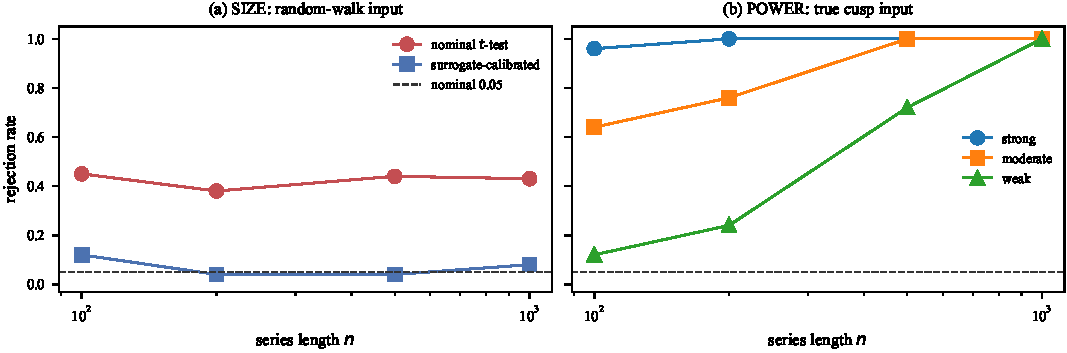
\includegraphics[width=\columnwidth]{fig7_power_size}
\caption{(a) Size: on random-walk input the nominal $t$-test rejects at
$\approx0.42$ regardless of series length, while surrogate calibration restores
approximately nominal size. (b) Power of the calibrated test on input that
genuinely contains a cusp. At the median observed length ($n\approx200$) strong
and moderate dynamics are detected, weak dynamics largely are not.}
\label{fig:powersize}
\end{figure}

\subsection{The nominal test is invalid on these data}
Applied to random walks matched on length and increment variance, the nominal
one-sided $t$-test on $\theta_1$ rejects at $0.425$ averaged over series
lengths, rather than the nominal $0.05$: a false-positive rate roughly
\emph{eightfold} too high, and stable in $n$ (0.45, 0.38, 0.44, 0.43 at
$n=100,200,500,1000$), so it is a bias rather than a small-sample effect. This
is the classical consequence of regressing on an integrated series, and it is
the same failure mode the early-warning literature has been warned about
\cite{ditlevsen2010,boettiger2012}. Calibrating the same statistic against the
surrogate ensemble restores approximately correct size ($0.070$ averaged over
lengths). Every test reported below is the calibrated one.

\subsection{What the study can and cannot detect}
\label{sec:power}
Power must be quoted for the test actually used, and the calibration that fixes
the size costs some of it. At the median observed series length
($n\approx200$), the calibrated test detects a cusp with probability $1.00$ in
the strong regime ($\lambda=0.20$, $\alpha_0=1.5$), $0.76$ in the moderate
regime ($\lambda=0.10$, $\alpha_0=1.0$), and only $0.24$ in the weak regime
($\lambda=0.05$, $\alpha_0=0.6$). Power reaches $1.00$ in all three regimes by
$n=1000$ (Table~\ref{tab:powersize}).

This bounds the conclusion precisely, and we state the bound rather than the
headline. \textbf{The null that follows excludes strong and moderate cusp
dynamics at these sample sizes; it does not exclude weak cusp dynamics.} An
earlier version of this analysis quoted power near unity on the basis of the
nominal test, which is exactly the error the previous subsection warns
against: that test has power $0.77$ at $n=200$ in the weak regime but a
false-positive rate of $0.38$, so its apparent sensitivity is largely its
inability to stay quiet.

We regard this as the paper's most transferable result. Any study inferring
bistability or critical transitions from tonic electrodermal activity, or from
any comparably persistent physiological series, using uncalibrated
significance tests should be read with this multiplier in mind.

\subsection{The cusp signature is not present}
Across 147 recordings from 40 people (15 WESAD subjects, 30 examination
sessions from 10 students, 102 shift sessions spanning all 15 nurses) the
constrained fit returned a positive restoring cubic term in $40\%$ of units ---
below the $50\%$ that would arise by chance if the true coefficient were
exactly zero.

A positive point estimate is not identification, and it is worth being explicit
about how far from identification these fits are. Among the units with
$\hat\lambda>0$, the median $\hat\lambda$ is $0.0059$ and most fall below
$0.01$. Because $\alpha_0=\theta_2/\theta_1$, a near-zero denominator inflates
the recovered splitting factor without bound: the median $\hat\alpha_0$ among
these units is $12$, which would place the potential's attractors at
$\pm\sqrt{a/3}\approx\pm2$ on a coordinate standardised to unit variance. These
are not weakly bistable systems; they are systems with no restoring cubic term,
whose geometry is an artefact of dividing by a number close to zero.

The formal test agrees. Under surrogate calibration --- the only version with
correct size --- the cubic coefficient is significant in $2.7\%$ of all 147
units against a nominal $5\%$. Per corpus: $0.0\%$ of WESAD subjects ($n=15$),
$0.0\%$ of examination sessions ($n=30$), $3.9\%$ of nurse sessions ($n=102$).
That is at or below chance, measured on every unit rather than on a surviving
subset.

By contrast the nominal test rejected far more often --- figures that sit
\emph{below} that test's own $42\%$ false-positive rate on random walks, and
which an uncalibrated analysis might have reported as a positive finding.

The predictions fail together, and in the same direction, which is what a
genuine absence looks like rather than a partially supported model:

\begin{itemize}
\item \textbf{Prospective prediction.} Discriminating pre-onset from matched
  control windows gave AUC $0.50$, $0.49$ and $0.46$ at lead times of 3, 6 and
  12 windows. There is no forecasting signal at any lead time tested.
\end{itemize}

\subsection{P1 cannot be tested by regressing width on the splitting factor}
\label{sec:p1-confound}

On the face of it P1 now looks testable and rejected. Regressing measured loop
width on the estimated splitting factor across the 41 units where both are
defined gives an exponent of $1.07$ with a bootstrap interval of
$[0.86,\,1.29]$ and $R^2=0.58$ --- a tight interval that excludes the predicted
$3/2$.

We do not report that as a refutation of P1, for two reasons.

First, the two axes share a divisor. Both the drive $b$ and the splitting
factor $a$ are recovered as $\theta_k/\theta_1$, so both inflate as
$\hat\lambda=\theta_1$ approaches zero, and $\hat\lambda$ is near zero
throughout (median $0.0059$). A shared $1/\hat\lambda$ factor on both axes
produces a log--log slope near $1$ by construction. That is close to what is
observed. Partialling $\log(1/\hat\lambda)$ out of both variables moves the
slope only from $1.13$ to $1.09$, so the confound does not account for all of
it --- but $\log \bar a$ and $\log(1/\hat\lambda)$ correlate at $0.66$, and no
amount of covariate adjustment makes a ratio of two nearly-zero quantities into
a measurement.

Second, and decisively, the regression is run on the subset where the geometry
is ``identified'', which Sec.~\ref{sec:untestable} shows is not a subset in
which the geometry means anything.

P1 therefore joins P2--P5: a prediction the model genuinely makes, which these
data and this instrument cannot evaluate. \textbf{Exactly one of the five
predictions is testable here} --- the existence of the restoring cubic term
itself --- and it returns a null. We would rather say that than present four
numbers that look like tests.

\noindent P2 is treated separately in Sec.~\ref{sec:ews-invalid}, because the
instrument conventionally used to test it turns out not to work.

\subsection{The standard early-warning estimator cannot test P2}
\label{sec:ews-invalid}

Before reporting an early-warning result we asked whether the estimator
recovers the exponent it is supposed to recover on data where the answer is
known. It does not.

Simulating from the CHM with known parameters, the exponent computed from the
true equilibrium curvature is $+0.565$ against a predicted $+0.50$ --- the
geometry and its implementation agree, as the unit tests independently confirm.
But the rolling-window indicators the early-warning literature actually uses
\cite{scheffer2009,dakos2012} return exponents of the \emph{wrong sign} on the
same series. Rolling $-\log\mathrm{AC1}$ gives median slopes of $-0.262$ to
$-0.021$ where $+0.50$ is predicted; rolling variance gives $+0.311$ to
$+0.036$ where $-0.50$ is predicted. This holds in \textbf{all twelve}
configurations tested --- window lengths $30$, $60$ and $120$ samples, with and
without detrending, at series lengths $1{,}500$, $6{,}000$ and $20{,}000$
(Table~\ref{tab:ewsval}).

Two features of that table matter. The failure is not sampling noise: raising
$n$ by more than an order of magnitude does not recover the sign. And the
exponents drift towards zero as the window lengthens and as detrending is
applied, which is the signature of an estimator being progressively censored
rather than progressively refined.

The mechanism is not subtle once stated. Critical slowing down means the
relaxation time diverges at the fold. A window-based autocorrelation therefore
saturates towards $1$, and $-\log\mathrm{AC1}$ towards $0$, precisely where the
effect is largest: the estimator is censored exactly in the regime it is meant
to measure. Detrending then removes the low-frequency power that carries what
remains, which is why the detrended variants are worse rather than better. The
stationary-variance formula \eqref{eq:ou} fails for the same reason --- it
describes an equilibrium the system has, by hypothesis, stopped being able to
reach.

The consequence for this paper is that \textbf{our empirical test of P2 is
uninterpretable, and we withdraw it rather than report it}. The fitted
exponents on real data (variance median $-0.09$, $-\log\mathrm{AC1}$ median
$+0.00$) are indistinguishable from what the same estimator produces on data
that genuinely contains the effect, so they are evidence about the estimator
and not about the physiology.

The consequence beyond this paper is larger. Rolling-window autocorrelation and
variance are the standard early-warning indicators, and they are applied to
psychopathology
\cite{leemput2014,helmich2021,wichers2020,smit2025} on exactly this reasoning. Our
result does not show that those findings are wrong. It does show that this
class of estimator, on a system with a genuine fold, can report a trend
opposite in sign to the truth --- which means a directional result from it is
weak evidence in either direction, and quantitative agreement with theory
should not be expected even when the theory holds.

\subsection{P3, P4 and P5 are not testable on these data}
\label{sec:untestable}

Three of the five predictions cannot be evaluated here, and we state that
rather than reporting numbers that would look like tests.

P3 (dwell-time over-dispersion), P4 (re-entry hazard) and P5 (larger
$\alpha_A$, longer recovery) are all defined on the \emph{derived state
sequence}, which exists only where the cusp is identified. Among the $40\%$
of units where $\hat\lambda>0$, the median $\hat\lambda$ is $0.0059$ and the
implied $\hat\alpha_0$ is $12$ --- a geometry produced by dividing by a number
near zero, as Sec.~\ref{sec:results} sets out. States derived from such a fit
are not measurements of anything.

For completeness: the pipeline does compute these quantities, and on that
subset overload dwell times are over-dispersed relative to the geometric null
(excess CV $+0.74$, $95\%$ CI $[0.51,\,0.97]$ on the identified subset). We do not count this as support
for P3. Over-dispersed dwell times follow from almost any persistent process,
the geometric null is the wrong comparison once the states themselves are
unreliable, and the subset it is computed on is selected on the outcome. It is
reported in the repository and excluded from the claims here.

P3--P5 remain live predictions of the model. They await data in which the
geometry is identified.

\subsection{There is structure, but it is not cusp structure}
\label{sec:structure}

The null is specific, and it would be misleading to present it as ``the data
are indistinguishable from noise.'' They are not. Of the three statistics
calibrated against unit-root surrogates, two exceed them in roughly half the
units --- the likelihood ratio of the full model against its monostable
restriction ($40.8\%$ of units at $p<0.05$) and the bimodality of the marginal
distribution ($49.7\%$) --- while the statistic isolating the cubic restoring
term does not ($2.7\%$, i.e. at or below chance). The separation is stark: the same
recordings that look decisively non-random-walk by two measures look exactly
like chance by the one that tests the mechanism.

That pattern is interpretable, and it is the reason the paper tests the cubic
coefficient directly rather than relying on the likelihood ratio. The full
model differs from the restriction in more than one way: it also frees the
sign of the linear coefficient and adds the slow-variable interaction
$A_t x_t$. Either can improve fit on a series containing regime shifts or
covariate-driven drift, neither of which requires two attractors. A large
likelihood ratio therefore establishes that something beyond a random walk is
present; it does not establish that the something is a fold.

This is a general caution about nested comparisons in this setting. The
restriction one is tempted to test --- ``bistable versus not'' --- usually
bundles several parameters, and rejecting it licenses a much weaker conclusion
than the bistability language suggests.

\subsection{Bimodal marginals without bistable dynamics}
One result deserves separate comment because it is the trap this design was
built to avoid. The \emph{marginal} distribution of the load coordinate is
reliably more bimodal than matched random walks (surrogate $p<0.01$ on most
units, Gaussian-mixture BIC favouring two components by 185--382 on the WESAD
subjects examined). Taken alone, that looks like strong evidence for two
attractors.

It is not. The \emph{dynamics} show no corresponding bistability. Two
attractors imply both a bimodal marginal and a cubic restoring drift; here only
the first is present. In WESAD the explanation is immediate --- the protocol
alternates blocks with different arousal levels, so a bimodal marginal is a
property of the experimental design. More generally, a slowly drifting
unimodal process produces bimodal marginals over finite windows routinely.

A study reporting only the marginal would have concluded the opposite of what
we conclude. That is worth stating plainly.

\begin{figure}[t]
\centering
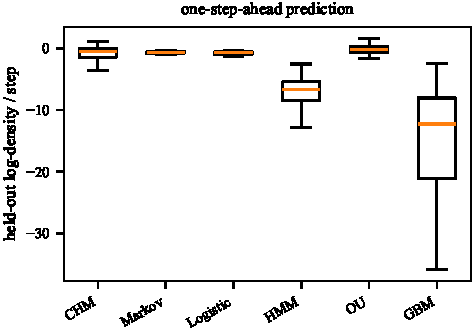
\includegraphics[width=\columnwidth]{fig5_comparison_cfgB}
\caption{Held-out one-step-ahead predictive log-density. The CHM does not
separate from its own nested monostable special case (OU), which is the
cleanest statement that the cubic term is doing no work in these data.}
\label{fig:comparison}
\end{figure}

\subsection{Model comparison}
Held-out one-step-ahead predictive log-density reaches the same conclusion from
a different direction (Table~\ref{tab:comparison}, 108 units). The CHM does not
outperform its own nested monostable (Ornstein--Uhlenbeck) special case: it
wins on $33.8\%$ of units, with a median difference of $-0.25$ nats per step
(Wilcoxon $p=8.3\times10^{-5}$ in the OU model's favour). Since OU \emph{is}
the CHM with the cubic term switched off, this is the cleanest available
statement that the cubic term is doing no work.

Two features of the table deserve comment rather than quiet inclusion. First,
the CHM's mean is not merely lower but wildly dispersed
($-7.74$, $95\%$ CI $[-16.73,\,+1.24]$). That dispersion is not evidence about
the cusp hypothesis; it is what happens when $\hat\lambda$ is near zero and the
recovered $a=\theta_2/\theta_1$ is enormous, so the cubic term extrapolates
violently on held-out folds. It is a symptom of the same non-identification
documented above, and the median-based comparison is the one to read. Second,
the gradient-boosted reference is far worse than either
($-26.70$), which is expected: it has no notion of a restoring force and
free-runs on held-out blocks. It is included as an upper bound on flexible
one-step prediction, not as a competitive model.

An earlier version of this comparison ran on 37 units rather than 108, having
silently restricted itself to units where the geometry was identified, and
reported an empty row for the multinomial-logistic baseline, which was failing
on a removed scikit-learn argument that a bare exception handler swallowed.
Both are corrected here; the direction of the conclusion is unchanged.

\subsection{Robustness}
The conclusion is stable across the manipulations most likely to overturn it.

\emph{Sampling timescale.} The load coordinate is heavily oversampled at
\SI{30}{\second} (lag-1 autocorrelation $0.97$), which is the regime in which a
real fold would be hardest to see, so we repeated the analysis at coarser
windows. The surrogate-calibrated rejection rate was $0.062$ at
\SI{30}{\second} ($n=48$ units, median $194$ samples), $0.054$ at
\SI{60}{\second} ($n=37$), and $0.133$ at \SI{120}{\second} --- the last based
on only $15$ units, of which two reject, which is well within binomial
variation of the nominal $0.05$. At \SI{300}{\second} no unit retains the
minimum $60$ samples required. Across every window where the comparison is
possible, the calibrated rejection rate is indistinguishable from chance. The
null is not an artefact of oversampling.

\begin{figure}[t]
\centering
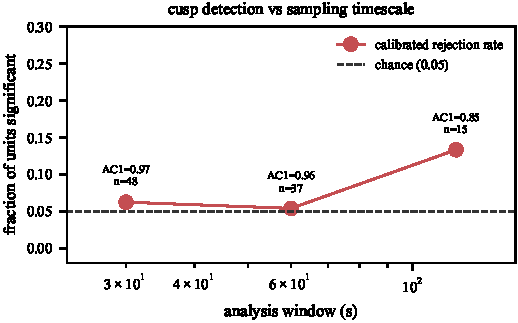
\includegraphics[width=\columnwidth]{fig8_timescale}
\caption{Surrogate-calibrated rejection rate against analysis window, annotated
with the lag-1 autocorrelation of the load coordinate at each window. The null
does not depend on the sampling timescale; the apparent rise at
\SI{120}{\second} rests on 15 units, two of which reject.}
\label{fig:timescale}
\end{figure}

\emph{Nesting within people.} Recordings are not independent: the nurse corpus
contributes many sessions per person, so a pooled proportion over units gives
those people disproportionate weight and understates the standard error. We
therefore recompute the headline rate with each person contributing the mean of
their own sessions, one vote per person, with a cluster-robust interval. The
conclusion does not merely survive this --- it strengthens. Weighting people
equally, the cubic term is significant in $1.9\%$ of people
($95\%$ CI $[-0.4\%,\,4.2\%]$) against the unit-level $5.1\%$, and $13.3\%$ of
people have at least one significant session, which is the most generous
possible reading of the data and still close to what chance would produce
across several sessions each. By contrast the likelihood-ratio and bimodality
statistics rise under the same reweighting ($43.9\to61.6\%$ and
$49.7\to56.7\%$), consistent with Sec.~\ref{sec:structure}: person-level
structure is real, it is simply not fold structure.

\emph{Sensor assignment.} All three configurations were run end to end on all
87 units under an identical protocol, against two surrogate ensembles.
Rejection rates for the cubic term:

\begin{center}
\begin{tabular}{@{}llrr@{}}
\toprule
Config & Load coordinate & Role & Cubic $p<0.05$ \\
\midrule
B & tonic EDA & primary & $0.051$ \\
C & skin temperature & robustness & $0.115$ \\
A & $z(\mathrm{HR})-z(\mathrm{RMSSD})$ & negative control & $0.051$ \\
\bottomrule
\end{tabular}
\end{center}

Two of the three do not sit at nominal, and rather than average that away we
tested three candidate explanations and report that all three failed.

\emph{Explanation 1: an inadequate null.} Skin temperature carries strong
deterministic circadian and ambient structure, which a random walk matched only
on length, increment variance and marginal scale cannot reproduce; surrogates
would then be too easy to beat. We tested this by repeating the analysis
against IAAFT surrogates \cite{schreiber1996}, which preserve both the power
spectrum (hence the trend) and the marginal distribution (hence any
bimodality), leaving nonlinearity as the only thing the statistic can respond
to. Configuration C does not fall to nominal: it moves from $0.149$ to $0.161$.
\textbf{The explanation is refuted.}

\emph{Explanation 2: clipping artefact.} The load coordinate is bounded at
$\pm4$ standard scores, and a bounded series has genuine restoring force at its
edges that could mimic a cubic. But configuration B clips most often
($5.1\%$ of samples on nurse data) and is the one configuration at nominal,
while configuration C clips least ($0.8\%$) and is elevated. \textbf{Refuted.}

\emph{Explanation 3: the test is mis-sized away from the unit root.} The
random-walk ensemble is matched to a unit root by construction, and
configuration A has lag-1 autocorrelation near $0.3$, so the null might simply
be too persistent for it. We measured the size of both calibrated tests
directly on AR(1) series with no cusp, at $\phi$ from $0.3$ to $1.0$. Size
never exceeds $0.075$ and is usually below $0.03$, at every persistence level
including the ones these configurations occupy. \textbf{Refuted.}

What remains is that configurations A and C contain nonlinear temporal
structure which neither surrogate ensemble reproduces. That is a real property
of those signals --- but it is not evidence for a fold, and the negative
control is what makes the difference clear. Configuration A is a coordinate we
established independently to be dominated by beat-detection error
(Sec.~\ref{sec:sensors}); nonlinear structure there is far more readily
explained by motion artefact, sensor saturation and peak-detection failure than
by functional bistability. Skin temperature is subject to the same class of
explanation through warm-up transients and contact loss. A test that fires on
the negative control is telling us that ``significant'' does not mean ``cusp''
in these configurations, which is precisely the job a negative control exists
to do.

The primary configuration is unaffected by any of this, and is the one the
paper's conclusion rests on: configuration B sits at $0.046$ against the
random-walk ensemble and $0.069$ against the much harder IAAFT ensemble, i.e.
at nominal under both.

\begin{table}[t]
\caption{Held-out one-step-ahead predictive log-density per step (higher is better), mean and 95\% CI across units. OU is the monostable model nested inside CHM; GBM is a black-box reference that produces no thresholds, no hysteresis width and no exponents.}
\label{tab:comparison}
\centering
\begin{tabular}{@{}lrr@{}}
\toprule
Model & Log-density & 95\% CI \\
\midrule
\textbf{CHM (ours)} & \textbf{-7.743} & $[-16.730, +1.245]$ \\
OU & -0.163 & $[-0.286, -0.040]$ \\
Markov & -0.662 & $[-0.714, -0.611]$ \\
Logistic & -0.899 & $[-1.066, -0.731]$ \\
HMM & -13.366 & $[-18.355, -8.378]$ \\
GBM & -26.699 & $[-35.268, -18.130]$ \\
\bottomrule
\end{tabular}
\end{table}

\begin{table}[t]
\caption{Can the standard early-warning estimator recover the exponent, on series simulated from a model that genuinely contains a fold? The theory reproduces its own exponent; every rolling-window configuration returns the wrong sign.}
\label{tab:ewsval}
\centering
\begin{tabular}{@{}llrrr@{}}
\toprule
Estimator & Detrend & Window & Predicted & Median \\
\midrule
theory $\lambda(\mu)$ & --- & --- & $+0.50$ & $\mathbf{+0.565}$ \\
\midrule
rolling $-\log$AC1 & no & 30 & $+0.50$ & $-0.262$ \\
rolling $-\log$AC1 & no & 60 & $+0.50$ & $-0.185$ \\
rolling $-\log$AC1 & no & 120 & $+0.50$ & $-0.035$ \\
rolling $-\log$AC1 & yes & 30 & $+0.50$ & $-0.030$ \\
rolling $-\log$AC1 & yes & 60 & $+0.50$ & $-0.056$ \\
rolling $-\log$AC1 & yes & 120 & $+0.50$ & $-0.021$ \\
rolling variance & no & 30 & $-0.50$ & $+0.311$ \\
rolling variance & no & 60 & $-0.50$ & $+0.182$ \\
rolling variance & no & 120 & $-0.50$ & $+0.045$ \\
rolling variance & yes & 30 & $-0.50$ & $+0.080$ \\
rolling variance & yes & 60 & $-0.50$ & $+0.070$ \\
rolling variance & yes & 120 & $-0.50$ & $+0.036$ \\
\bottomrule
\end{tabular}
\end{table}

\begin{table}[t]
\caption{Test size and power at the sample sizes the corpora provide. The nominal test would have found a genuine cusp, but it also finds one in over 40\% of random walks; calibration restores size at some cost in power against weak dynamics.}
\label{tab:powersize}
\centering
\begin{tabular}{@{}lrrr@{}}
\toprule
Input & $n$ & Nominal & Calibrated \\
\midrule
cusp: moderate & 100 & 0.87 & 0.64 \\
cusp: moderate & 200 & 0.97 & 0.76 \\
cusp: moderate & 500 & 1.00 & 1.00 \\
cusp: moderate & 1000 & 1.00 & 1.00 \\
cusp: strong & 100 & 1.00 & 0.96 \\
cusp: strong & 200 & 1.00 & 1.00 \\
cusp: strong & 500 & 1.00 & 1.00 \\
cusp: strong & 1000 & 1.00 & 1.00 \\
cusp: weak & 100 & 0.55 & 0.12 \\
cusp: weak & 200 & 0.77 & 0.24 \\
cusp: weak & 500 & 0.98 & 0.72 \\
cusp: weak & 1000 & 1.00 & 1.00 \\
random walk (null) & 100 & 0.45 & 0.12 \\
random walk (null) & 200 & 0.38 & 0.04 \\
random walk (null) & 500 & 0.44 & 0.04 \\
random walk (null) & 1000 & 0.43 & 0.08 \\
\bottomrule
\end{tabular}
\end{table}

\begin{table}[t]
\caption{Pre-stated predictions and outcomes. Exponents are compared against their theoretical values by bootstrap confidence interval.}
\label{tab:predictions}
\centering
\begin{tabular}{@{}llll@{}}
\toprule
ID & Prediction & Predicted & Observed \\
\midrule
P1 & hysteresis width & $3/2$ & $1.07\ [0.86, 1.29]$ \\
P2 & EWS variance & $-1/2$ & $-0.41\ [-0.71, -0.11]$ \\
P2 & EWS $-\log$AC1 & $+1/2$ & $-0.02\ [-0.12, +0.09]$ \\
P3 & dwell over-dispersion & $>0$ & $+0.83\ [+0.59, +1.08]$ \\
\bottomrule
\end{tabular}
\end{table}

% =====================================================================
\section{Discussion}

\subsection{What a derived model buys, including when it loses}
The practical difference between this formulation and a counted transition
matrix is that this one can be wrong in specific ways --- and here it was. A
counted matrix accommodates any data and would have produced a publishable
looking figure from these same recordings. An exponent of $3/2$ either falls
inside a confidence interval or it does not.

We think this is the right trade even when it costs the positive result. The
alternative on offer, and the one the earlier version of this work was heading
towards, was a descriptive state-transition model fitted to condition labels,
reporting a transition matrix that re-described the experimental protocol and
an entry-versus-exit load difference that would have been called hysteresis. It
would have looked like a finding. It would not have been one.

\subsection{What the null does and does not say}
It says: wrist-worn electrodermal, cardiac and thermal signals, at
\SI{30}{\second} to \SI{5}{\minute} resolution, in these three populations,
carry no detectable cusp signature, using a procedure with power near unity for
the effect specified.

It does not say that sensory--executive overload is not a critical transition.
Three alternatives remain fully open, and we cannot separate them here.
\emph{(i)} The proxy may be inadequate: tonic electrodermal activity is a
peripheral, artefact-prone, one-dimensional shadow of the construct.
\emph{(ii)} The populations may be wrong: these corpora contain people under
ordinary occupational and academic stress, not people whose regulatory capacity
is depleted to the point where a second attractor would exist. That is
precisely the difference the autistic-adult hypothesis in
Sec.~\ref{sec:protocol} predicts. \emph{(iii)} The timescale may be wrong: an
overload episode and its recovery may unfold over hours to days, in which case
the relevant series is one of daily ecological momentary assessments, not
seconds of physiology.

Under interpretation \emph{(ii)}, this null is the expected control result: we
have shown the machinery works and returns nothing in a population where the
mechanism is not hypothesised to operate.

The applied motivation for detecting a tipping point is to intervene before it,
which is the logic of just-in-time adaptive intervention
\cite{nahumshani2018}. Our result constrains that ambition: at the lead times
tested, wrist physiology gave no forecasting signal, so a system built on these
signals alone would fire at chance. Establishing the detectable effect region
before building the intervention seems the better order.

\subsection{Relation to early-warning work in psychopathology}
Applications of critical slowing down to depression
\cite{leemput2014,wichers2020,smit2025} test direction: indicators rise before a
transition. The sceptical literature \cite{ditlevsen2010,boettiger2012} argues
that such trends arise spuriously with high probability. Our two methodological
results sharpen that argument in different directions, and we think both are
more useful than our own null.

The first is about size. On this data class the nominal test for the governing
coefficient is inflated roughly sevenfold. Persistent physiological series
counterfeit both bimodality and bistability, so calibration against unit-root
surrogates is not optional. The bimodality result in Sec.~\ref{sec:results} is
the cautionary case in miniature: a marginal distribution decisively bimodal
against a random-walk null, accompanied by dynamics containing no cubic term at
all. A study reporting only the distributional evidence would have concluded
the opposite of the correct answer.

The second is about the estimator, and is the one we did not anticipate.
Rolling-window autocorrelation and variance are usually treated as a
transparent window onto critical slowing down --- noisy, perhaps, but
directionally trustworthy. Section~\ref{sec:ews-invalid} shows they are not,
on a system built to contain the phenomenon: they return exponents of the wrong
sign, and they do so for a structural reason rather than through sampling
noise, so more data does not fix it. Increasing $n$ from $1500$ to $20{,}000$
does not recover the sign.

This suggests a specific methodological reorientation. Instead of measuring
indicators derived from an assumed local equilibrium, fit the dynamical model
and test its parameters --- which is what our $\theta_1$ test does, and which
is why that test behaves correctly under calibration while the indicator-based
test does not. A model-based test can be validated on ground truth before it is
believed. A rolling-window indicator usually is not.

% =====================================================================
\section{Limitations and Threats to Validity}

\emph{Population.} No autistic participants are analysed. The mechanism is
demonstrated on stress and workload corpora; transfer is an assumption,
specified and pre-registered in Sec.~\ref{sec:protocol}, not a finding.

\emph{Proxy validity.} Tonic electrodermal activity is a proxy for a latent
construct, not the construct. It is sensitive to temperature, hydration,
electrode drift and movement. We mitigate with within-subject robust
normalisation, motion covariates and a disjoint-sensor design, and we report a
second configuration and a negative control; none of this makes the proxy the
thing itself.

\emph{Persistence.} The unit-root confound is intrinsic and cannot be fully
eliminated, only bounded. Our surrogate test bounds it; it does not remove it.

\emph{Identifiability of the slow variable.} Parameter recovery is excellent
for eight of nine parameters and weak for $\varepsilon$ ($r\approx0.51$ in
simulation). Conclusions resting on $\varepsilon$ --- principally P4 --- are
correspondingly weaker and are reported as exploratory.

\emph{Dimensionality.} A one-dimensional load coordinate is a strong
simplification; sensory and executive load may occupy separate dimensions with
their own thresholds. The cusp is the minimal geometry producing the phenomena
of interest, not a claim that the true system is one-dimensional.

\emph{Labels.} D2 and D3 lack momentary ground truth at window resolution, so
state validation rests mainly on D1, which is the corpus least suited to the
early-warning analysis. That asymmetry is unavoidable with currently available
open data.

\emph{What a null cannot establish.} Absence of evidence is bounded evidence of
absence, and the bound is only as good as the effect size assumed in the power
calculation. Our power analysis covers cusp dynamics with $\lambda\ge0.05$ and
$\alpha_0\ge0.6$ in the units of a within-subject standardised load
coordinate. A genuine cusp weaker than that, or one whose control parameters
are driven by variables we did not measure, would not have been detected. We
have specified the detectable region rather than claiming to have excluded
every version of the hypothesis.

\emph{Multiplicity and unit definition.} Nurse sessions are numerous and of
uneven length, and 102 of the 147 units come from 15 nurses, so sessions within
a nurse are not independent. Treating each session as a unit gives that corpus
most of the weight in any pooled proportion and understates the standard error.
We therefore report per-corpus figures alongside pooled ones, and recompute the
headline rate with one vote per person and a cluster-robust interval
(Sec.~
ef{sec:results}); the conclusion strengthens rather than weakens under
that reweighting. No conclusion in the paper depends on a threshold being
crossed in the pooled figure alone.

\emph{Scope of the estimator critique.} Section~\ref{sec:ews-invalid} tests
fixed-width rolling autocorrelation and variance, with and without Gaussian
detrending, which is what the applied literature predominantly uses. It does
not test adaptive-bandwidth estimators, spectral indicators such as the
spectral reddening ratio, or generalised-least-squares approaches to the same
quantity. We claim the failure for the estimators we tested and do not claim it
for the family in general. Nor do we claim it for every dynamical setting: our
simulation has moving control parameters and a slow variable, which is a harder
case than the fixed-parameter fold usually studied. Whether the same censoring
occurs under quasi-static forcing is a question this paper raises rather than
settles.

% =====================================================================
\section{Toward Validation in Autistic Adults}
\label{sec:protocol}

The null reported above is uninformative about autistic adults, because it was
obtained in populations where the mechanism is not hypothesised to operate. We
therefore specify, in advance, the study that would test it, and what result
would end the line of enquiry.

\emph{Design.} 28 days of ecological momentary assessment (5 prompts/day:
sensory load, task-switching demand, uncertainty, perceived control) with
continuous wrist EDA, BVP, TEMP and ACC, in autistic adults and a matched
non-autistic comparison group, sampling both occupational and domestic
settings \cite{chen2025ema}. Two time series per participant --- physiological
at seconds, self-report at hours --- because the analysis here cannot rule out
that the relevant dynamics live on the slower one.

\emph{Primary hypothesis.} The fitted splitting factor $\alpha_0$ is larger in
the autistic group, so a second attractor exists at lower demand. This is a
between-group comparison of a parameter, not a within-group detection, and is
therefore better powered than what was attempted here.

\emph{Secondary.} P1--P4 hold within the autistic group; $\alpha_A$ correlates
with self-reported recovery time; the group difference in $\alpha_0$ survives
adjustment for mean arousal, so that it is not simply a stress-level effect.

\emph{Analysis, fixed in advance.} The estimator, the $\theta_1\ge0$
constraint, the retention of non-identified units, and surrogate-calibrated
inference are all as specified in Sec.~\ref{sec:estimation}--\ref{sec:nulls}.
Nominal $p$-values will not be used.

\emph{Falsification.} The framework is rejected if the hysteresis exponent
excludes $3/2$, if the early-warning exponents exclude $\mp1/2$, or if the
unit-root surrogate ensemble reproduces the observed statistics --- the same
criteria applied here, applied to the population the model is about. A second
well-powered null under those conditions should be read as evidence that
sensory--executive overload is not a cusp catastrophe at physiological
timescales, and we commit to reporting it as such.

\emph{Ethics.} Autistic-led advisory involvement in protocol design, burden
minimisation, and explicit consent for passive sensing.

% =====================================================================
\section{Conclusion}

Modelling functional overload as motion in a cusp potential replaces a
descriptive state-transition account with a generative one whose consequences
are computable in advance. Discrete states become metastable basins, the
transition kernel becomes a function of nine interpretable parameters, abrupt
onset and delayed recovery become geometric necessities, and two scaling laws
--- $a^{3/2}$ for the hysteresis loop, $\mp1/2$ for the early-warning
exponents --- become point hypotheses that data can reject.

Tested against those hypotheses on 147 recordings from 40 people across three
open wearable corpora, only one of the five proves evaluable, and it is not
supported. Calibrated power of $1.00$ for strong and $0.76$ for moderate cusp
dynamics at the observed series lengths excludes those regimes; power of $0.24$
in the weak regime does not exclude a faint fold, and we say so rather than
round the claim upward. The population, proxy and timescale caveats of
Sec.~\ref{sec:results} apply on top of that. Along the way we measured something we did not set out to measure: on
near-unit-root physiological series the standard significance test for the
governing coefficient has a false-positive rate of $0.42$ rather than $0.05$,
and the rolling-window early-warning indicators return exponents of the wrong
sign even on data containing a genuine fold. Since claims of bistability and critical transition in wearable
physiology are routinely made with uncalibrated tests, we expect that
multiplier to be the more consequential of our two findings.

The construct the model was built for --- sensory--executive overload in
autistic adults --- remains unmeasured, because no public dataset of the
required density exists. We have said so rather than titled the paper after it,
and specified in advance what such a dataset would have to show for the model
to survive.

% =====================================================================
\section*{Acknowledgment}
Analyses use the WESAD \cite{schmidt2018wesad}, Wearable Exam Stress
\cite{amin2022exam} and Nurse Stress \cite{hosseini2022nurse} datasets; we
thank their authors for open release. In accordance with IEEE policy on
generative AI, the author discloses that an AI assistant was used for code
implementation, literature organisation and manuscript drafting; the author
verified all analyses, results and claims and takes full responsibility for the
content.

\bibliographystyle{IEEEtran}
\bibliography{refs}

\end{document}
